\subsection{Обоснование необходимости проводимого исследования}
Настоящая дипломная работа исследует алгоритмы поиска смещений по парам изображений основываясь на дифференциальном алгоритме Лукаса-Канаде. На основе полученных векторных полей смещений можно строить карты поверхностной деформации твердого тела.

Целью дипломной работы является разработка программного обеспечения (ПО) для оценки деформаций поверхностей твёрдых тел, а также проведение исследований алгоритмов и методов как на модельных, так и на реальных оптических изображениях.

\subsection{Планирование комплекса работ по разработке программного обеспечения}
Основными задачами планирования работ являются:

\begin{itemize}
\item определение объёма предстоящих работ;
\item распределение объёма работ на взаимосвязанные последовательные этапы;
\end{itemize}

\begin{itemize}
\item установление сроков выполнения работ;
\item определение необходимых, для выполнения планируемых работ денежных, материальных и трудовых ресурсов.
\end{itemize}
При выполнении дипломной работы было задействовано два человека:

\begin{itemize}
\item руководитель (рук.);
\item разработчик (разр.).
\end{itemize}

Руководитель выполняет контроль выполнения различных этапов работ, согласованность этапов выполнения работ между собой, корректирует действия разработчика, дает рекомендации по выполнению тех или иных работ. Разработчик реализует тот объем работ, который установлен руководителем в соответствие с техническим заданием.

Месячный оклад студента в ТУСУР равен 10483 рублей, с учетом 20 рабочих дней в месяце, и 8 часового рабочего дня, стоимость одного часа работ равна 65,51 рублей. Месячный оклад руководителя к.т.н., доцента в университете равен 14800 рублей, с учетом 24 рабочих дней, и 6 часового рабочего дня, стоимость одного часа работ равна 102,8 рубля.

График выполнения работ приведен в таблице \ref{tab:job_is_done_1}.

\begin{table}[!ht]
\caption{График выполнения работ}
\centering
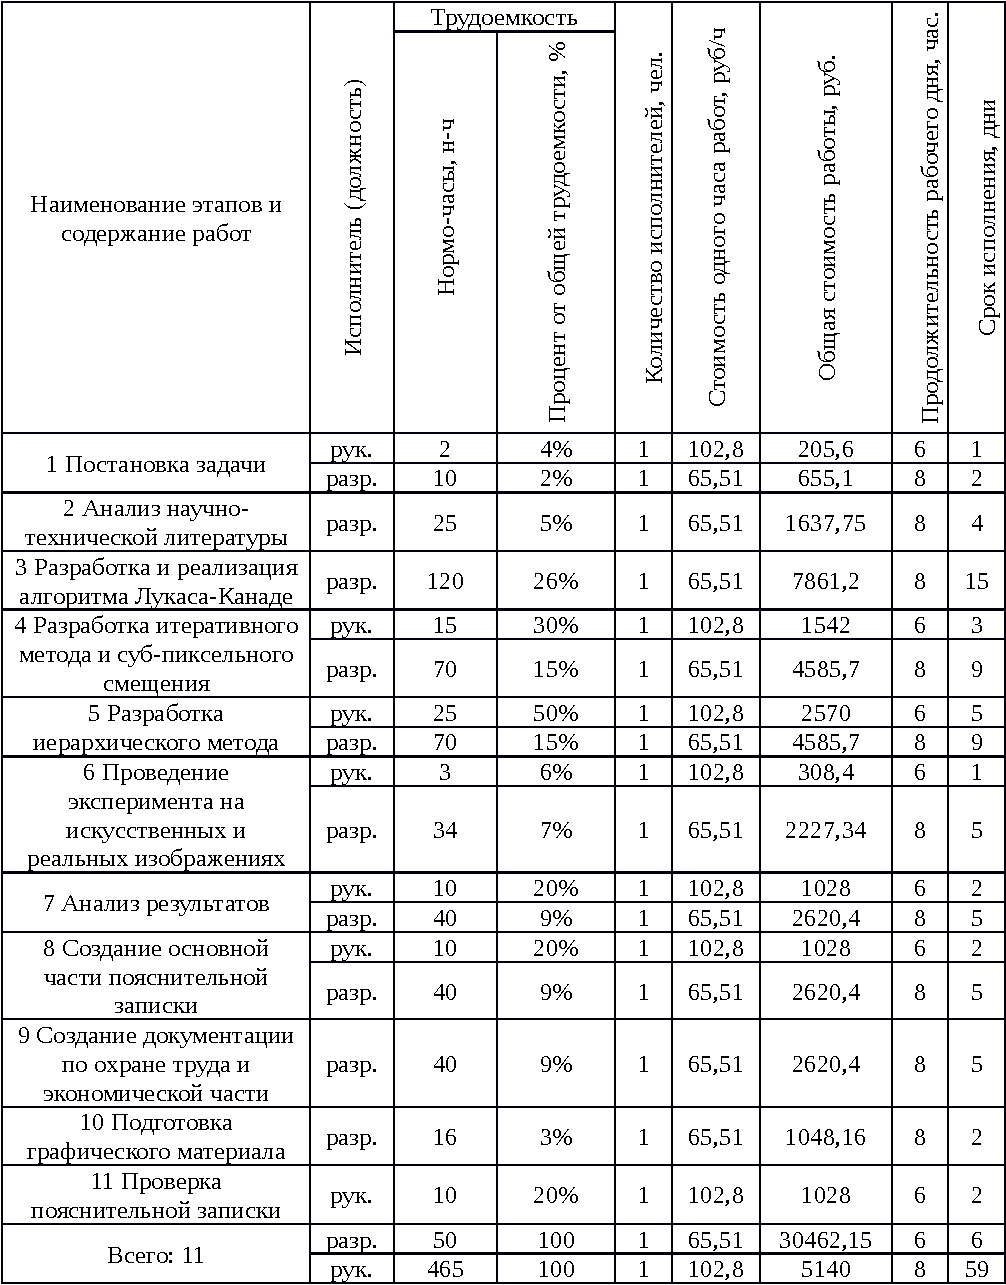
\includegraphics[page=1, width=1\linewidth]{econom_table.pdf}
\label{tab:job_is_done_1}
\end{table}

Зная длительность цикла каждого этапа и возможность их параллельно-последовательного выполнения, можно рассчитать срок завершения планируемых работ и составить ленточный и сетевой графики плана их выполнения. Поскольку работа не требует большого состава исполнителей, то ограничимся ленточным графиком планирования, представленным в виде таблицы \ref{tab:eco_2}.

\begin{table}[!ht]
\caption{Ленточный график загрузки участников работ}
\centering
\includegraphics[page=2, width=1\linewidth]{econom_table.pdf}
\label{tab:eco_2}
\end{table}

\begin{table}[!ht]
\caption{Календарный график загрузки участников}
\centering
\includegraphics[page=3, width=1\linewidth]{econom_table.pdf}
\label{tab:eco_3}
\end{table}

\subsection{Определение сметной стоимости проекта}
\subsubsection{Общие положения}

Смета затрат для данной работы состоит из расходов, которые включают в себя следующие статьи:

\begin{itemize}
\item затраты на оборудование и амортизацию;
\item расходы на оплату труда и отчисления на социальные нужды;
\item затраты на основные и вспомогательные материалы;
\item затраты на электроэнергию.
\end{itemize}
\subsubsection{Затраты на оборудование и амортизацию}

Основным оборудованием при проведении работы являются компьютер и принтер, которые постановлением Правительства Российской Федерации от 1.01.02 г. N 1 отнесены ко второй амортизационной группе – «имущество со сроком полезного использования свыше 2 лет до 3 лет включительно». Месячная норма амортизации составляет 2,8\% и для компьютера, и для принтера.

Результаты расчётов амортизационных отчислений приведены в таблице \ref{tab:eco_4}.

\begin{table}[!ht]
\caption{Смета затрат на оборудование}
\centering
\includegraphics[page=4, width=1\linewidth]{econom_table.pdf}
\label{tab:eco_4}
\end{table}

\subsubsection{Расходы на оплату труда и отчисления на социальные нужды}

Статья затрат учитывает выплаты по заработной плате за выполненную работу, исчисленные на основании тарифных ставок и должностных окладов в соответствии с принятой в организации-разработчике системой оплаты труда. В этой статье также отражаются премии, надбавки и доплаты за условия труда, оплата ежегодных отпусков, выплата районного коэффициента и некоторые другие расходы. Отчисления на социальные нужды учитывают страховые взносы.

Результаты расчета расходов на оплату труда участников проекта представлены в таблице \ref{tab:eco_5}.

\begin{table}[!ht]
\caption{Расчет расходов на оплату труда участников проекта}
\centering
\includegraphics[page=5, width=1\linewidth]{econom_table.pdf}
\label{tab:eco_5}
\end{table}

\subsubsection{Затраты на основные и вспомогательные материалы}

Статья включает расходы по приобретению и доставке основных и вспомогательных материалов, необходимых для опытно-экспериментальной проработки решения, для изготовления макета или опытного оборудования. Сюда включаются и стоимость необходимых материалов для изготовления образцов и макетов, и материалов необходимых для оформления требуемой документации.

Размер транспортно-заготовительных расходов (ТЗР), определяемый в процентах от стоимости, примем 10\%. Стоимость вспомогательных материалов принимается 10\% от стоимости основных материалов с учетом ТЗР. Результаты расчёта стоимости материалов представлены в \ref{tab:eco_6}.

\begin{table}[!ht]
\caption{Расчёт затрат на основные и вспомогательные материалы}
\centering
\includegraphics[page=6, width=1\linewidth]{econom_table.pdf}
\label{tab:eco_6}
\end{table}

\subsubsection{Расходы на электроэнергию}

Статья включает затраты по электроэнергии на технологические нужды. В настоящее время тариф на электроэнергию для населения г. Томска на 2015 год составляет 2,7 руб./ кВт ч. Введенный приказом от 26.12.2014 {\textquotedbl} №6/9 (691) «О тарифах на электрическую энергию для населения и потребителей, приравненных к категории население по Томской области на 2015 год», принятый департаментом тарифного регулирования Томской области.

Результаты расчётов приведены в \ref{tab:eco_7}.

\begin{table}[!ht]
\caption{Затраты на электроэнергию}
\centering
\includegraphics[page=7, width=1\linewidth]{econom_table.pdf}
\label{tab:eco_7}
\end{table}

\subsubsection{Накладные расходы}

Расчет накладных расходов сведем в \ref{tab:eco_8}.

\begin{table}[!ht]
\caption{Накладные расходы}
\centering
\includegraphics[page=8, width=1\linewidth]{econom_table.pdf}
\label{tab:eco_8}
\end{table}

\subsubsection{Сводная смета затрат}

На основании всех произведённых расчётов составим сводную смету затрат на выполнение работы в виде таблицы \ref{tab:eco_9}.

\begin{table}[!ht]
\caption{Сводная смета затрат}
\centering
\includegraphics[page=9, width=1\linewidth]{econom_table.pdf}
\label{tab:eco_9}
\end{table}

\subsection{Научно-технический эффект}
Количественная оценка научно-технического уровня может быть произведена путем расчета результативности участников разработки по формуле:

{\centering\color{black}
 $\text{\textcyrillic{К}}_{\mathit{\text{\textcyrillic{н}}\text{\textcyrillic{у}}}}=\sum _{i=1}^n\left(\text{\textcyrillic{К}}_{\mathit{\text{\textcyrillic{д}}\text{\textcyrillic{у}}}}{\cdot}d_i\right)$,
\par}

где\ $K_\textit{ну}$ – коэффициент научного или научно-технического уровня;

%$K_\textit{ду}\textit{\textsubscript{i}}$ – коэффициент достигнутого уровня $\textit{i}{}$-го фактора;

%\textit{d}\textit{\textsubscript{i}}\textit{ }– значимость \textit{i}{}-го фактора;

\textit{n} – количество факторов.

Весовые коэффициенты \textit{d} для каждого из факторов устанавливались экспертным путем. При этом сумма коэффициентов значимости по всем факторам равна единице. Коэффициенты достигнутого уровня факторов также установлены экспертным путем.

\begin{table}[!ht]
\caption{Оценка научно-технического уровня разработки}
\centering
\includegraphics[page=10, width=1\linewidth]{econom_table.pdf}
\label{tab:eco_10}
\end{table}
Рассчитанный коэффициент научно-технической результативности равен 0,7075. Полученное значение достаточно высоко, что говорит об эффективности проведенных работ выше среднего, однако отмечается необходимость дальнейшего развития проекта для достижения завершенности полученных результатов.

\subsection{1.5 Социальный эффект}
Гипотетический социальный эффект заключается в улучшении результатов исследований, проводимых в лаборатории механики полимерных композиционных материалов СО РАН, которые могут использовать программное обеспечение оценки деформации твердых тел, и усилении научного потенциала.